
% Compile with XeLaTeX

\documentclass[12pt]{article}
\usepackage{fontspec}
\usepackage[a4paper,bindingoffset=0.2in,%
            left=0.75in,right=0.75in,top=0.75in,bottom=0.75in,%
            footskip=.25in]{geometry} 
\usepackage{graphicx}
\graphicspath{ {./images/} }
\usepackage{float}
\usepackage{hanging}
\usepackage{hyperref}

\setmainfont{Times New Roman}
\title{Group 4 - Housing Price Prediction}
\date{\today}
\author{
Erik Alvstad, Lance Halsted, Ruiyi He, Ashley Li, Abdullah Mohammed\\William Schmidt, Qilin Wang, Cai Xu, Ruyi Yang
}
 
\begin{document}
\maketitle

\section*{Introduction}
\href{https://github.com/wilschmidtt/Group-4-Housing-Prices}{Github Link}
\\
\par \qquad The housing market contributes between 15-18\% of the United States GDP, depending on the year (NAHB). Such a relatively high contribution, coupled with the necessity of such products makes datasets composed of explanatory variables (\emph{id est} size, number of bedrooms, number of bathrooms, et cetera) and their sale price, both easy to obtain and quite substantial. Dean De Cock at Truman State University collected 2930 real estate sale observations, from the city of Ames, Iowa, with 80 explanatory variables (De Cock). The dataset has since been used as an educational tool for undergraduate regression courses. With this in mind, our team has set out to create a machine learning algorithm to accurately predict the sale price of a house from these explanatory variables based on this dataset.

\section*{Background}
\par \qquad The basic premise of machine learning is to produce a model that accurately predicts relationships in data from a statistical sample of a population. Producing a model that does not fully capture the relationships in the sample such that the model cannot predict those of the population well is referred to as underfitting. Producing a model that predicts the sample well by describing “noise” in the data, rather than describing overall trends, and therefore, cannot accurately predict those in the population is referred to as overfitting. The goal of machine learning, therefore, is to produce a model that is detailed enough to prevent underfitting, while also reducing the detail such that overfitting does not occur.
\par Linear regression analysis is a statistical method of determining the linear relationship between two variables. The most basic of these is simple linear regression, wherein constants \emph{$\beta_0$}  and \emph{$\beta_1$} are selected such that some error function of the difference between \emph{$y = \beta_0 + \beta_1x$} and the actual values of \emph{y} is minimized. Multiple linear regression is a methodology by which the same procedures are performed, however, several explanatory variables ($x_{1}, x_{2}$, etc) are analyzed: \emph{$y=\beta_{0}+\beta_{1}x_{1}+\beta_{2}x_{2}+......+\beta_{n}x_{n}+ \epsilon$} (Pedregosa \emph{et al.}).
\par There are several methods for determining the constants that reduce the error to its global minimum. While the absolute global minimum can be calculated with linear algebra, with large datasets this becomes unfeasible and gradient descent methodologies become preferential. Among the most common methodologies in the study of machine learning include ordinary least-squares regression, stochastic gradient descent regression, ridge-regularized regression, lasso-regularized regression, support vector regression, and polynomial regression.
\par Gradient descent methodologies, follow a simple procedure. First, random values for each constant are chosen. Then, expected values are calculated for some portion of the dataset. The error function’s derivative is calculated, and the constants are changed to move the error function down its gradient (Pedregosa \emph{et al.}). This is repeated until a local minimum is found.
\par Ordinary least-squares (OLS) regression is an analytical methodology of determining the global optimum for a linear regression. It uses matrix multiplication, and, therefore, suffers from a large time complexity (Pedregosa \emph{et al.}).
\par Stochastic gradient descent (SGD) is a methodology that seeks to improve the speed of OLS regression. SGD uses a numerical approach compared to the analytical approach used in OLS. SGD uses a learning rate hyperparameter, a, to determine the size of steps in moving toward the minimum: \emph{$w_j=w_j-\alpha\frac{\delta{RSS}}{\delta{w_j}}$}. However, SGD is not guaranteed to give an optimal solution since it may find a local minimum instead of the global minimum.
\par Polynomial regression is a special case of linear regression where an nth-degree polynomial is used to model the relationship between the n independent variables and the target variable (Sharma). The model function is linear with respect to the model weights. The formula, therefore, is \emph{$y=\beta_0+\beta_{1}x+\beta_{2}x^2+\beta_{3}x^3+...+\beta_{n}x^n$}. Higher-order polynomial regression can lead to overfitting of the training data.
\par Ridge-regularized regression is a methodology that seeks to prevent overfitting by minimizing the values of the constants. This is achieved by appending the sum of squares of the regression constants to the error function, multiplied by an additional hyperparameter (Pedregosa \emph{et al.}).
\par Lasso-regularized regression is a methodology almost identical to ridge-regularized regression, however, instead of appending the sum of squares of the regression constants, the sum of the regression constants is appended (Pedregosa \emph{et al.}).
\par Support Vector Regression (SVR) uses the same principle as SVM, but applies it to regression problems instead of classification problems. In SVR, the best fit line is a hyperplane that has a maximum number of points within a threshold distance. The SVR kernel can be either linear, polynomial or nonlinear. Due to SVR’s fit-time complexity, it is not suitable for very large datasets (Raj).

\section*{Literature Review}
\par \qquad The prediction of sale price has numerous applications in real-world service industries. Online shopping services may want to determine the best price for a given individual shopper, and investors may want to predict if and when a stock price may rise and fall. The housing market is a market in which the features of the product for sale vary wildly, and price has many explanatory variables. As such, it is a prime application of machine learning algorithms. It is almost certain that linear regression analyses provide effective means of determining the sale price of the house, though they are often used in conjunction with other methodologies.
\par As a problem that requires the use of supervised learning, regression analyses are often used for their prediction. In Truong \emph{et al.’s} analysis of housing prices in Beijing, it was found that a regression analysis of the sale price with features as explanatory variables was satisfactory with a large sample of 300,000 observations. Similarly, in an analysis of housing prices in Melbourne City, Australia, students at Macquarie University used linear and polynomial regression to produce a satisfactory model using a data set of about 35,000 samples with 21 explanatory variables. (The Danh Phan). 
\par Ensemble machine learning techniques are often found to be best for this problem. In Varma \emph{et al.’s} analysis of machine learning algorithms, it was found that an optimal machine learning methodology for house sale prices in Mumbai, India, was an ensemble methodology, featuring regression and neural networks. Ensemble methodologies have been found to perform better than pure regressions (Varma \emph{et al.}).
\par In Yichen Zhou’s masters thesis, a linear regression as well as a lasso regularized linear regression are performed on the De Cock dataset and tested for accuracy. OLS regression analysis was found to perform better with this dataset than Lasso-regularized least squares regression (Zhou).

\subsection{Dataset}
\par \qquad Our team obtained a subset of the original dataset from Kaggle. Kaggle is a public dataset repository. The dataset involved had 1460 instances, each with 80 different attributes. Of the attributes, 28 were numeric, and 52 were categorical.
\par The dataset’s attributes were titled with strings with 12 characters or less. For the sake of reducing confusion, the attributes and their meanings are summarized in the \emph{Attributes} section below.

\subsection{Attributes}
\begin{enumerate}
\setlength{\itemsep}{-1mm}
\item ID: which instance was recorded (irr)
\item MSSubClass: the building class (cat)
\item MSZoning: the zoning classification (cat)
\item LotFrontage: the length of street connected to the perimeter (cat)
\item LotArea: the lot size in square feet (num)
\item Street: the type of road access (cat)
\item Alley: the type of alley access (cat)
\item LotShape: the lot shape (cat)
\item LandContour: flatness (cat)
\item Utilities: the type of utilities available (cat)
\item LotConfig: the lot configuration (cat)
\item LandSlope: the slope of the property (cat)
\item Neighborhood: the location (cat)
\item Condition1: the proximity to various railroads and road features (cat)
\item Condition2: the proximity to various railroads and road features (cat)
\item BldgType: the type of structure (cat)
\item HouseStyle: the style of the structure (cat)
\item OverallQual: the quality of the material and finish (cat)
\item OverallCond: the condition (cat)
\item YearBuilt: the original construction date (cat)
\item YearRemodAdd: the date of any remodeling (irr)
\item RoofStyle: the style of roofing (cat)
\item RoofMatl: the roofing material (cat)
\item Exterior1st: the first exterior covering (cat)
\item Exterior2nd: the first exterior covering (cat)
\item MasVnrType: the masonry veneer (cat)
\item MasVnrArea: the masonry veneer area in square feet (num)
\item ExterQual: the exterior quality (cat)
\item ExterCond: the exterior condition (cat)
\item Foundation: the type of foundation (cat)
\item BsmtQual: the height of the basement (cat)
\item BsmtCond: the condition of the basement (cat)
\item BsmtExposure: the exposure of the basement walkout (cat)
\item BsmtFinType1: the rating of the first basement finish (cat)
\item BsmtFinSF1: the area of the first basement finish (num)
\item BsmtFinType2: the rating of the second basement finish (cat)
\item BsmtFinSF2: the area of the second basement finish (num)
\item BsmtUnfSF: the square feet of the unfinished basement area (num)
\item TotalBsmtSF: the total square feet of basement area (num)
\item Heating: the type of heating (cat)
\item HeatingQC: the heating quality and condition (cat)
\item CentralAir: whether there was central air conditioning on the property (cat)
\item Electrical: the type of electrical system (cat)
\item 1stFlrSF: the area of the first floor in square feet (num)
\item 2ndFlrSF: the area of the second floor in square feet (num)
\item LowQualFinSF: the area of low quality finish in square feet (num)
\item GrLivArea: the living area above ground in square feet (num)
\item BsmtFullBath: the amount of full bathrooms in the basement (num)
\item BsmtHalfBath: the amount of half bathrooms in the basement (num)
\item FullBath: the amount of full bathrooms above ground (num)
\item HalfBath: the amount of half bathrooms above ground (num)
\item Bedroom: the amount of bedrooms above ground (num)
\item Kitchen: the amount of kitchens above ground (num)
\item KitchenQual: the quality of the kitchens (cat)
\item TotRmsAbvGrd: the total amount of non-bathroom rooms above ground (num)
\item Functional: the home functionality (cat)
\item Fireplaces: the amount of fireplaces (num)
\item FireplaceQu: the quality of the fireplaces (cat)
\item GarageType: the location of the garage (cat)
\item GarageYrBlt: the year built of the garage (irr)
\item GarageFinish: the type of interior finish of the garage (cat)
\item GarageCars: the size of the garage in car capacity (num)
\item GarageArea: the size of the garage in square feet (num)
\item GarageQual: the quality of the garage (cat)
\item GarageCond: the condition of the garage (cat)
\item PavedDrive: the amount of driveway paved (cat)
\item WoodDeckSF: the area of wood deck in square feet (num)
\item OpenPorchSF: the area of open porch in square feet (num)
\item EnclosedPorch: the area of enclosed porch in square feet (num)
\item 3SsnPorch: the area of three season porch in square feet (num)
\item ScreenPorch: the area of screen porch in square feet (num)
\item PoolArea: the area of pool (num)
\item PoolQC: the quality of the pool (cat)
\item Fence: the quality of the fence (cat)
\item MiscFeature: miscellaneous features unlisted elsewhere (cat)
\item MiscVal: the value of the miscellaneous feature (num)
\item MoSold: the month sold (cat)
\item YrSold: the year sold (cat)
\item SaleType: the type of sale (cat)
\item SaleCondition: the condition of the sale (cat)
\end{enumerate}

\section*{Analysis}
\par \qquad The attributes listed were not statistically independent. Several simple linear regressions performed between attributes yielded correlation values far above 0.5. The largest of which was between \emph{GarageArea} and \emph{GarageCars}, which had a correlation of 0.88. Some other notable attribute correlations include \emph{GarageYrBlt} and \emph{YearBuilt}, with a correlation of 0.83, in addition to \emph{1stFlrSF} and \emph{TotalBsmtSF}, with a correlation of 0.82. Indeed, the largest of the correlations usually emerged due to the attributes in question having similar, if not identical meanings (\emph{GarageArea} and \emph{GarageCars} both state how large the garage of the instance is, albeit with different units). There are few, if any, attributes that have nonzero correlations, and most fall around 0.20.
\par The attributes were, for the most part, normally distributed. The distributions of the numeric attributes do not deviate far from a normal distribution. With how extensive the numeric attributes were, and the target variable itself being numeric, the dataset in question was an adequate candidate for regression analysis.

\begin{figure}[H]
\centering
\renewcommand{\thefigure}{1.1}
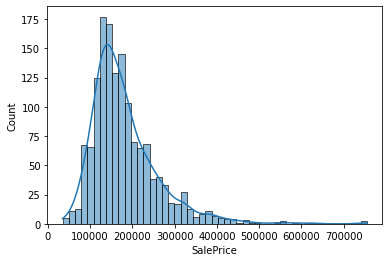
\includegraphics{fig1.3.png}
\caption{A histogram depicting the distribution of the \emph{SalePrice attribute}}
\end{figure}

\par The target variable, \emph{SalePrice}, had a right-skewed normal distribution. As seen in Figure 1.1, there is a single peak, and few, if any, irregularities in the data.

\section*{Methodology}
\par \qquad Our team preprocessed the dataset and trained and tested the model using the Jupyter Notebook running Python 3. The libraries used included Numpy, Pandas, and SciKit-Learn. Numpy is an open-source Python library for numeric computation that was created in 2005. Pandas is an open-source Python library for data analysis that was created in 2008. SciKit-Learn is a Python library for machine learning that was created in 2007.

\subsection{Dataset Preprocessing}
\par \qquad The provided dataset underwent several transformations before it was used for model training. Heuristics were used to determine initial preprocessing steps, then the methodology was refined through experimentation.
\par The dataset was first converted into a Pandas dataframe. Next, the target variable was separated from the training variables. Then, each training variable was grouped into one of three categories: categorical variables, numeric variables, and irrelevant variables - listed as cat, num, and irr in the \emph{Attributes} section.
\par Categorical variables were variables in which two or more non-ordinal categories were possible for each instance in the dataframe. Such variables were encoded via one-hot encoding. For some categorical variables, “NA” values were supported and indicated that the feature in question was not present.  For such variables, “NA” entries were converted to the string “None” to avoid Pandas treating them as missing values. For all remaining categorical features, “NA” values were processed as missing entries. Furthermore, the numeric variables \emph{LotFrontage} and \emph{MasVnrArea} used “NA” to denote a value of 0. In these cases, all “NA” values were converted to 0 to avoid Pandas treating them as missing. 
\par Numeric variables were normalized to their respective z-scores, following a simple normal distribution. Outliers were systematically removed by dropping any instance of a numeric variable falling 3.5 standard deviations or greater from the mean. This threshold was determined through experimentally observing the effect it had on model performance. Both removing outliers and preserving the robustness of the model were the two main factors taken into account.
\par Variables that were deemed irrelevant were those that did not add useful information to the model - such as the ID of the house - or highly correlated variables. Correlation was observed using the ‘pandas.DataFrame.corr’ method. Irrelevant features were simply dropped from the dataframe.
\par Once each of the explanatory variables had been effectively transformed, the categorical, numeric, and target data frames were concatenated into a single object. From here, a .csv file was saved locally that would be used for model training.

\subsection{Model Training}
\par \qquad A total of six different models were trained and subsequently tested. An OLS regression, a SGD linear regression, a ridge-regularized linear regression, a lasso-regularized linear regression, a support vector regression, and a polynomial (quadratic) regression were each performed on the dataset. Each model was performed with grid-search hyperparameter tuning and was subject to 10-fold cross validation.

\subsection{Model Testing}
\par \qquad Each model was tested for its root-mean-squared error on the respective testing sets of the 10-fold cross validation, with the averages calculated and compared. The model with the smallest average root-mean-squared error was selected as the final model.

\section*{Results}

\begin{figure}[H]
\centering
\renewcommand{\thefigure}{2.1}
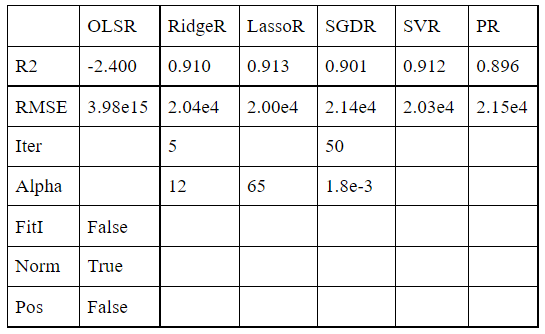
\includegraphics{2.1.png}
\caption{The average r-squared values and root-mean-squared errors of each optimized model, as well as the optimal hyperparameters: Iter is the number of iterations performed; Alpha is the alpha value for gradient descent; FitI fits the model to the intercept; Norm normalizes the data; Pos makes all the coefficients positive; empty cells mean that the hyperparameter is N/A.}
\end{figure}

\par \qquad After all of the procedures were performed, each of our models was tested, and their outputs are depicted in Figure 2.1.

\begin{figure}[H]
\centering
\renewcommand{\thefigure}{2.2}
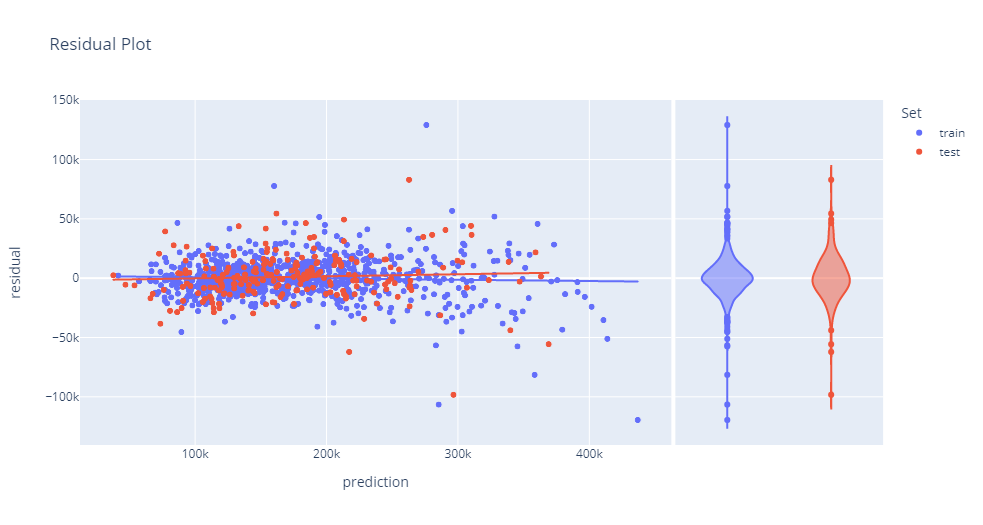
\includegraphics[width=\textwidth,height=\textheight,keepaspectratio]{2.2.png}
\caption{Residual plot for Lasso-regularized regression model}
\end{figure}

\par Since Lasso performed best, a residual plot of the predicted price vs the actual price in the test and training sets is depicted in Figure 2.2. Ideally, the residuals should be independent of the target variable and normally distributed. The Lasso residual plot has fairly good symmetry around the residual=0 axis, especially for houses that cost below \$350k. 

\section*{Discussion}
\par \qquad While most of the regression analyses performed had similar results, one of the major outliers was the OLS regression. It performed the worst, by far, with a root mean squared error of 3.98e15. While it is hard to say why this regression failed to produce the desired outcome, several hypotheses are possible. Perhaps the relationships that exist in the dataset are not strictly linear, and a linear regression is not applicable. Indeed, the polynomial regression, which, in this experiment, performed a quadratic regression analysis, did perform better than the OLS regression. Perhaps the optimal linear regression has very large coefficients that do not fit the population well. Ridge regularized linear regression does perform better than OLS regression, and ridge regularization is a methodology to prevent large coefficients in the model.
\par The polynomial regression performed quite well; 2.15e4 was a substantially lower RMSE than the OLS RMSE. Perhaps this is due to some of the relationships in the sample being quadratic rather than strictly linear. This may be the case, however, the polynomial regression was not best, and so, there may have been other problems with this regression that went unaddressed.
\par The stochastic gradient descent model performed well in this experiment. With a RMSE of 2.14e4, this model performed better than the OLS. Since the OLS is likely a global minimum, this would seem to mean that SGD found a local minimum with better performance than the OLS global minimum. As stated prior, this may be because the SGD had smaller coefficients relative to the OLS model.
\par The ridge regularization regression model performed better than the stochastic gradient descent model. Since the ridge regression is mainly used to prevent large coefficients from reducing the testing accuracy of regression models, the ridge regression’s success, relative to both the SGD and the OLS indicate that this factor is relevant to the dataset.
\par The SVR model performed very well. Ultimately, this may be due to its design; the methodology of determining the optimal hyperplane was different from the other regression methodologies. However, it was not the best.
\par The Lasso-regularization model performed best. With a r-squared value of 0.913 and a RMSE of 2.00e4, this function was substantially better than the SGD and the OLS, indicating that, at least for linear regressions, performing regularization functions to reduce coefficients is an optimal way of dealing with the sample size being as small as the De Cock dataset’s.

\section*{Conclusion}
\par \qquad The dataset that all of the models discussed were trained with had several significant problems: it was small and had several, highly-correlated attributes. These characteristics are all factors that increase the likelihood of large coefficients. The best model was the lasso-regularized linear regression, which was produced with a methodology that seeks to reduce the size of coefficients drastically. It is very likely that this was a major problem that each of the models faced. The OLS regression model performed the worst, and its regression is likely the global minimum of the training set.
\par With this dataset and with others, experts in the field of machine learning use linear regression techniques with neural networks and other ensemble models to determine relationships in housing prices (Varma \emph{et al.}). While these models are beyond the scope of this paper, it has been effectively shown that linear regression can be used as a single method for discovering these relationships.
\par While large datasets require vast computational power to produce optimal models, smaller datasets induce problems with overfitting that can only be overcome with sophisticated methodologies and hyperparameter selection. Collecting larger datasets remains the most effective way of improving the accuracy of machine learning models.

\section*{References}
\begingroup
\noindent
\vspace{-3em}
\setlength{\parindent}{-0.5in}
\setlength{\leftskip}{0.5in}
\setlength{\parskip}{10pt}

A. Varma, A. Sarma, S. Doshi and R. Nair, "House Price Prediction Using Machine Learning and Neural Networks," \emph{2018 Second International Conference on Inventive Communication and Computational Technologies (ICICCT)}, 2018, pp. 1936-1939, doi: 10.1109/ICICCT.2018.8473231.

Dean De Cock. “Ames, Iowa: Alternative to the Boston Housing Data as an End of Semester Regression Project” \emph{Journal of Statistics Education}, Volume 19, Number 3. 2011.

“House Prices - Advanced Regression Techniques.” \emph{Kaggle}, www.kaggle.com/c/house-prices-advanced-regression-techniques/overview.

“Housing's Contribution to Gross Domestic Product.” NAHB, www.nahb.org/News-and-Economics/Housing-Economics/Housings-Economic-Impact/Housings-Contribution-to-Gross-Domestic-Product.

Scikit-learn: Machine Learning in Python, Pedregosa \emph{et al.}, JMLR 12, pp. 2825-2830, 2011.

Sharma, Abhishek, Introduction to Polynomial Regression (with Python Implementation), Retrieved from https://www.analyticsvidhya.com/blog/2020/03/polynomial-regression-python/

Raj, Ashwin, Unlocking the True Power of Support Vector Regression - Using Support Vector Machine for Regression Problems. Retrieved from https://towardsdatascience.com/unlocking-the-true-power-of-support-vector-regression-847fd123a4a0

The Danh Phan, Housing Price Prediction Using Machine Learning Algorithms: The Case of Melbourne City, Australia, Retrieved from https://ieeexplore.ieee.org/abstract/document/8614000

Truong, Quang, \emph{et al.} “Housing Price Prediction via Improved Machine Learning Techniques.” Procedia Computer Science, vol. 174, Elsevier BV, 2020, pp. 433–442. Crossref, doi:10.1016/j.procs.

Zhou, Y. (2020). Housing Sale Price Prediction Using Machine Learning Algorithms. UCLA. ProQuest ID: Zhou\_ucla\_0031N\_18606. Merritt ID: ark:/13030/m5wh7xdt. Retrieved from https://escholarship.org/uc/item/3ft2m7z5

\endgroup

\end{document}